%%%%%%%%%%%%%%%%%%%%%%%%%%%%%%%%%%%%%%%%%
% Large Colored Title Article
% LaTeX Template
% Version 1.1 (25/11/12)
%
% This template has been downloaded from:
% http://www.LaTeXTemplates.com
%
% Original author:
% Frits Wenneker (http://www.howtotex.com)
%
% License:
% CC BY-NC-SA 3.0 (http://creativecommons.org/licenses/by-nc-sa/3.0/)
%
%%%%%%%%%%%%%%%%%%%%%%%%%%%%%%%%%%%%%%%%%

%----------------------------------------------------------------------------------------
%	PACKAGES AND OTHER DOCUMENT CONFIGURATIONS
%----------------------------------------------------------------------------------------

\documentclass[DIV=calc, paper=a4, fontsize=10pt, twocolumn]{scrartcl}	 % A4 paper and 11pt font size

\usepackage{lipsum} % Used for inserting dummy 'Lorem ipsum' text into the template
\usepackage{url}
\usepackage{natbib}
\usepackage[english]{babel} % English language/hyphenation
\usepackage[protrusion=true,expansion=true]{microtype} % Better typography
\usepackage{amsmath,amsfonts,amsthm} % Math packages
\usepackage[svgnames]{xcolor} % Enabling colors by their 'svgnames'
\usepackage[hang, small,labelfont=bf,up,textfont=it,up]{caption} % Custom captions under/above floats in tables or figures
\usepackage{booktabs} % Horizontal rules in tables
\usepackage{fix-cm}	 % Custom font sizes - used for the initial letter in the document
\usepackage{natbib}
\usepackage{sectsty} % Enables custom section titles
\allsectionsfont{\usefont{OT1}{phv}{b}{n} \fontsize{12}{12}} % Change the font of all section commands
\usepackage{hyperref}
\usepackage{float}
\usepackage{fancyhdr} % Needed to define custom headers/footers
\pagestyle{fancy} % Enables the custom headers/footers
\usepackage{lastpage} % Used to determine the number of pages in the document (for "Page X of Total")

% Headers - all currently empty
\lhead{}
\chead{\emph{Flying Etiquette: Get that baby out of here!}}
\rhead{}

% Footers
\lfoot{}
\cfoot{}
\rfoot{\footnotesize Page \thepage\ of \pageref{LastPage}} % "Page 1 of 2"

\renewcommand{\headrulewidth}{0.0pt} % No header rule
\renewcommand{\footrulewidth}{0.4pt} % Thin footer rule

\usepackage{lettrine} % Package to accentuate the first letter of the text
\newcommand{\initial}[1]{ % Defines the command and style for the first letter
\lettrine[lines=3,lhang=0.3,nindent=0em]{
\color{black}
{\textsf{#1}}}{}}
\usepackage{color}
\definecolor{purple}{rgb}{.4,0,.8}
\newcommand{\hh}[1]{{\color{magenta} #1}}
\newcommand{\st}[1]{{\color{purple} #1}}


%----------------------------------------------------------------------------------------
%	TITLE SECTION
%----------------------------------------------------------------------------------------

\usepackage{titling} % Allows custom title configuration

\newcommand{\HorRule}{\color{black} \rule{\linewidth}{1pt}} % Defines the gold horizontal rule around the title

\pretitle{\vspace{-50pt} \begin{flushleft} \HorRule \fontsize{15}{15} \usefont{OT1}{phv}{b}{n} \color{black} \selectfont} % Horizontal rule before the title

\title{Using the \texttt{ggmosaic} Package: Get That Baby Out of Here} % Your article title
 % This should probably reference geomnet. Don't want it to be too long though
\posttitle{\par\end{flushleft}\vskip 0em} % Whitespace under the title

\preauthor{\begin{flushleft}\large \vspace{-.5cm} \usefont{OT1}{phv}{b}{sl} \color{black}} % Author font configuration

\author{Haley Jeppson, } % Your name

\postauthor{\footnotesize \usefont{OT1}{phv}{m}{sl} \color{Black} % Configuration for the institution name
Iowa State University % Your institution

\par\end{flushleft} \vspace{-.5cm} \HorRule \vspace{-1cm}} % Horizontal rule after the title
\date{} % Add a date here if you would like one to appear underneath the title block

%----------------------------------------------------------------------------------------

\usepackage{Sweave}
\begin{document}
\Sconcordance{concordance:flying.tex:flying.Rnw:%
1 91 1 1 0 78 1 1 5 2 1 1 38 1 3 2 1 1 6 1 2 2 1 1 6 1 2 5 1 1 13 1 3 2 %
1 1 9 1 4 1 7 1 4 7 1 1 5 1 2 4 1 1 5 1 2 4 1 1 5 1 2 3 1 2 3 1 1 1 3 1 %
2 1 3 1 2 17 1}


\maketitle % Print the title

\thispagestyle{fancy} % Enabling the custom headers/footers for the first page

%----------------------------------------------------------------------------------------
%	ABSTRACT
%----------------------------------------------------------------------------------------

% The first character should be within \initial{}
\vspace{-1cm}
\initial{T}\textbf{he data analysis blog FiveThirtyEight commissioned a SurveyMonkey Audience poll for two days in August of 2014 that sought insight on common aggravating behaviors on flights to judge the perceived level of rudeness of those actions. The survey had 1,040 respondents (874 of whom had flown). Using a new way to visualize categorical data in \texttt{R} with \texttt{gglot2}, I attempt to examine the unspoken social contract we all encounter when we fly a little deeper.}
\initial{V}\textbf{isualizing multidimensional data can be cumbersome. There is a subtle complexity that arises from the hierarchical structure of the counts and proportions that are important for understanding the multivariate discrete distributions. In addition, graphical methods for categorical data and mixtures of qualitative and quantitative data are not well developed in comparison with what is available for numeric variables. Mosaic plots provide one possibility of visualizing multidimensional data and can be a powerful and easy option. However, while mosaic plots have been implemented in a variety of packages, the ordinary grammar of graphics does not support mosaic plots. With the R package ggmosaic, a custom ggplot2 geom designed for mosaic plots is implemented. In addition, ggmosaic creates plots that can be converted into interactive plotly graphs.}



%----------------------------------------------------------------------------------------
%	ARTICLE CONTENTS
%----------------------------------------------------------------------------------------
\section*{Introduction}

\par Is there a social contract we should all be following when flying? Who gets to use that extra arm rest? Is it okay to recline your seat or to bring your baby or child on board? Are people upset if the child is unruly and, like Donald Trump, wish to "get that baby out of here?" \citep{cnn} How often are you allowed to leave your seat before being perceived as rude? Does the occupant of the window seat reserve all rights to the window shade? And is it okay to switch seats for family, friends, or to an unsold seat?

\par To learn a little about people's opinions on what is considered to be rude behavior while on an airplane, FiveThirtyEight ran a SurveyMonkey Audience poll for two days in August of 2014.  \citep{fivethirtyeight} The survey had 1,040 respondents (874 of whom had flown) aged 18-60+ from across the county and asked twenty-six questions that ranged from background information regarding the respondent to feelings regarding potentially aggravating behavior one might encounter on an airplane. The data set is available from FiveThirtyEight's data git hub repository.

\par To explore the data a bit more, I used the \texttt{ggmosaic} package. The original analysis done by FiveThirtyEight focused primarily on the perceived rudeness of a behavior, one behavior at a time, or comparing the response "Very Rude" across all behaviors. By using a mosaic plot, multiple categorical counts can be viewed simultaneously which will provide a clearer view of the underlying data and allow for more comparisons to be made. We can perhaps gain more insight into how the seat recliner, the chatterbox, or the unruly child is perceived and how those perceptions may be related.

%------------------------------------------------

\section*{The \texttt{ggmosaic} package}

\par The \texttt{ggmosaic} package was designed to create visualizations of categorical data, and has the capability to produce bar charts, stacked bar charts, mosaic plots, and double decker plots. The main focus of this paper, however, will be on mosaic plots. A mosaic plot is a convenient graphical summary of the conditional distributions in a contingency table, and in a mosaic plot, the area of each graphical element is proportional to the underlying probability of that category. This allows us to easily visualize how the joint distribution is composed of the product of the conditional and marginal distributions -- which, in turn, allows us to see any association that may be occurring between the variables. Because the plot is constructed hierarchically, the ordering of the variables is very important.  There are many features that can be customized in \texttt{ggmosaic}, including the type of partitioning, the ordering of variables, conditioning or faceting, and the spacing between the categories.

\par While mosaic plots have been implemented in a variety of packages in R \citep{R2016}, the ordinary grammar of graphics does not support mosaic plots. However, with version 2.0.0 of `ggplot2` \citep{ggplot2}, a way for other R packages to implement custom geoms was introduced. With the R package ggmosaic, a custom ggplot2 geom designed for mosaic plots is implemented. The \texttt{ggmosaic} package can be installed from \url{https://github.com/haleyjeppson/ggmosaic}.


\par \texttt{ggmosaic} was created primarily using \texttt{ggproto} and the \texttt{productplots} package which was created by \citet{productplots}. They refer to their framework as product plots, alluding to the computation of area as a product of height and width, and the statistical concept of generating a joint distribution from the product of conditional and marginal distributions.

\par To begin, \texttt{ggmosaic} began as a geom extension of the \texttt{rect} geom with the data handling provided in the \texttt{productplots} package which calculates \texttt{xmin}, \texttt{xmax}, \texttt{ymin}, and \texttt{ymax} for the \texttt{rect} geom to plot.

\par Having a geom designed for mosaic plots does more than simply allow us to utilize the ggplot2 customization options such as faceting and layering, it allows for a \texttt{ggplotly()} hook so we can create interactive mosaic plots. Although the \texttt{ggplotly()} function translates most of the geoms bundled with the \texttt{ggplot2} package, it has no way of knowing about the rendering rules for custom geoms. The \texttt{plotly} package does, however, contain the infrastructure to provide translations of custom geoms to plotly. In \texttt{ggplot2}, many geoms are special cases of other geoms. For example,\texttt{geom\_line()} is equivalent to \texttt{geom\_path()} once the data is sorted by the \texttt{x} variable. \citet{carson} Because GeomMosaic can be reduced to the lower-level geom GeomRect, we were able to write a method for the \texttt{to\_basic()} generic function in \texttt{plotly}.


\par \texttt{ggmosaic} does not come without its own set of limitations and the main hurdle \texttt{ggmosaic} faces is that \texttt{ggplot2} is not capable of handling a variable number of variables. The current solution is to read in the variables \texttt{x1} and \texttt{x2} as \texttt{x = product(x1, x2)}. The \texttt{product} function creates a data frame that combines all of the variables listed which allows for it to pass \texttt{check\_aesthetics}, and then splits the variables back apart for the calculations.

\par The product function creates limitations for values the variables can take, and what the labels of variables can be. When the variables are combined, the values, variable name, and level are separated using ":", "-", and ".". For example, the \texttt{x} variable data is read is as \texttt{level-variable:value.level-variable:value}. If any of the variable names or values of the variable contain one of those 3 symbols, the function will break.

\par The aesthetics set up the formula that determines the how the joint distribution will be broken down. The following aesthetics can be set:

\begin{itemize}
\item weight: select a weighting variable
\item \texttt{x}: select variables to add to formula
    \begin{itemize}
    \item declared as \texttt{x = product(x1, x2, ...)}
    \end{itemize}
\item \texttt{fill}: select a variable to be filled
    \begin{itemize}
    \item if the variable is not also called in \texttt{x}, it will be added to the formula in the first position
    \end{itemize}
\item \texttt{conds} : select a variable to condition on
\end{itemize}


\par These values are then sent through `productplots` functions to create the formula for the desired distribution: \texttt{weight $\sim$ fill $+$ x $|$ conds }

\par The other parameters that can be set include the \texttt{offset} and the \texttt{divider}. When there is a variable with many categories, it may be of interest to decrease the size of the spacing between the spines. This can be achieved by declaring \texttt{offset =}. The default setting is \texttt{offset = 0.01}. There are two main ways to partition the area - into bars or into spines. When the area is partitioned into bars, the height is proportional to value and the width equally divides the space. Bars can be arranged horizontally ("hbar") or vertically ("vbar"). Alternatively, the space can be partitioned into spines, where the width is proportional to value, height occupies full range. Spines are space filling and can be arranged horizontally ("hspine") or vertically ("vspine"). In \texttt{ggmosaic}, the type of partitioning desired can be specified by setting \texttt{divider = " "}. The default divider for one variable is "hspine".
When more than one variable is to be considered, a type of partition needs to be selected for each variable. By selecting \texttt{divider = mosaic()}, the default, or \texttt{divider = ddecker()}, the correct number of partitions will be selected. For example, if three variables were to be plotted, the default, \texttt{divider = mosaic()}, would partition the plot with spines in alternating directions, beginning with a horizontal spine, i.e. \texttt{divider = c("hspine", "vspine", "hspine")}. It is also an option to manually select the type of partition that will be used for each variable, i.e. \texttt{divider = c("hbar", "vspine", "hspine")}. It should be noted that the first partition in the vector will be the last partition made in the plot. As mentioned above, when no divider is declared, the default \texttt{divider = mosaic()} will begin with a horizontal spine and alternate directions with each subsequent variable.

\par Using mosaic plots to visualize this data will allow for the hierarchical structure of the counts and proportions, which is important for understanding the multivariate discrete distributions, to be seen.

%-----------------------------------------------------------------------------
\section*{Visualizing the data}

\par I began by taking a look at who is flying and how frequently they fly. In addition to answering questions about common aggravating behaviors, the respondents answered questions regarding their demographics. Some of the demographic types of questions asked included age, gender, household income bracket, education level and region.

\par Figure ~\ref{fig: who1} was created by first dividing the space into horizontal spines each representing the proportion of respondents within that household income bracket. We can view these horizontal spines in the final product and they will answer questions such as, "what proportion of the respondents have a household income of under \$100,000?" The next step was to split each horizontal spine into vertical spines, which were subsequently filled with different colors,  representing how frequently one flew. This plot can be used to answer questions such as "what proportion of those that have a household income of under \$24,999 flies a few times per month?"



\setkeys{Gin}{width=0.45\textwidth}
\begin{figure}[h!]
\caption{Who is flying?}
\centering
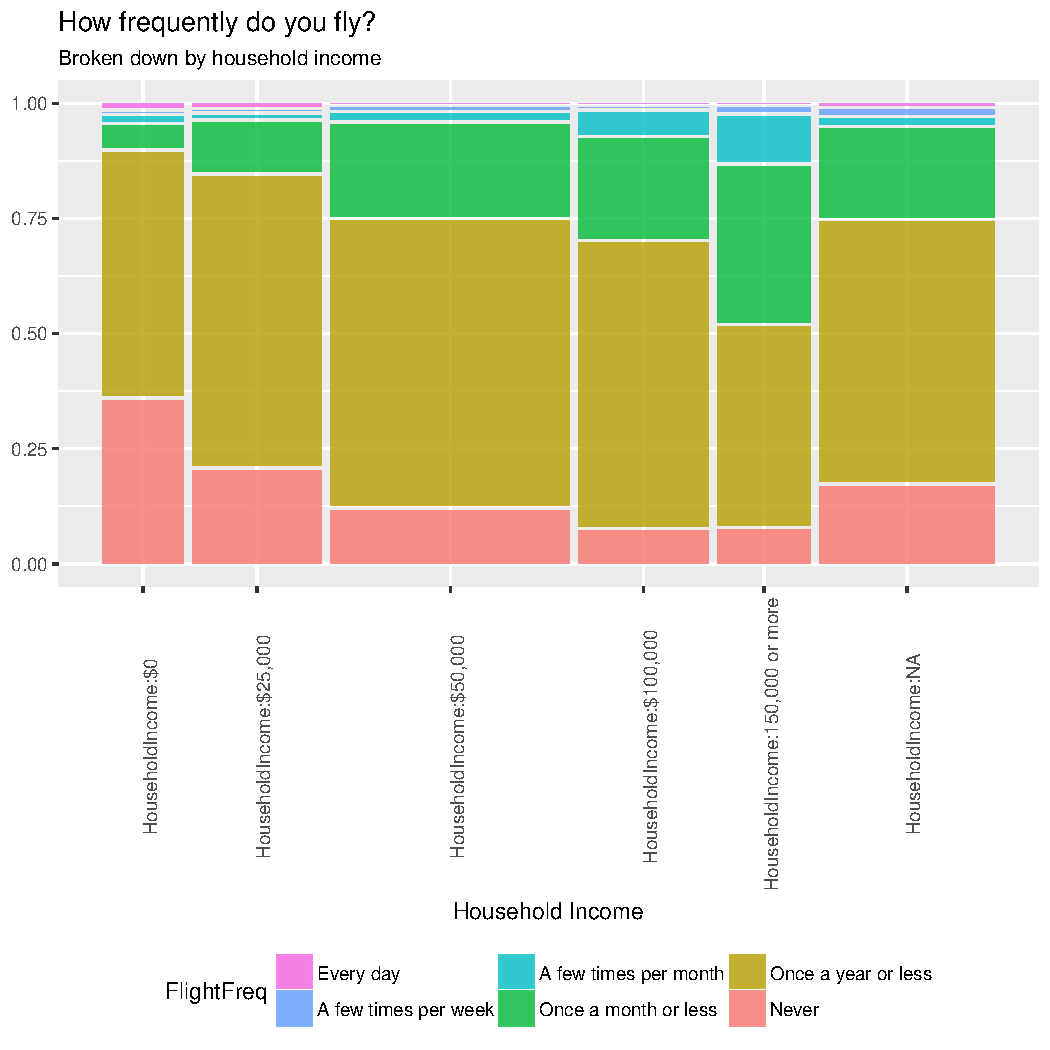
\includegraphics{flying-who1}
\label{fig: who1}
\end{figure}

\par From Figure ~\ref{fig: who1} we can see that the largest majority of the survey participants fall within the household income bracket of \$50,000-99,000, and that as household income increases, the more likely one is to frequently fly. Even more interesting, the few participants that responded that they flew every day were of the two lower income brackets or chose to not respond to the question.


\begin{figure}[h!]
\caption{Who is flying?}
\centering
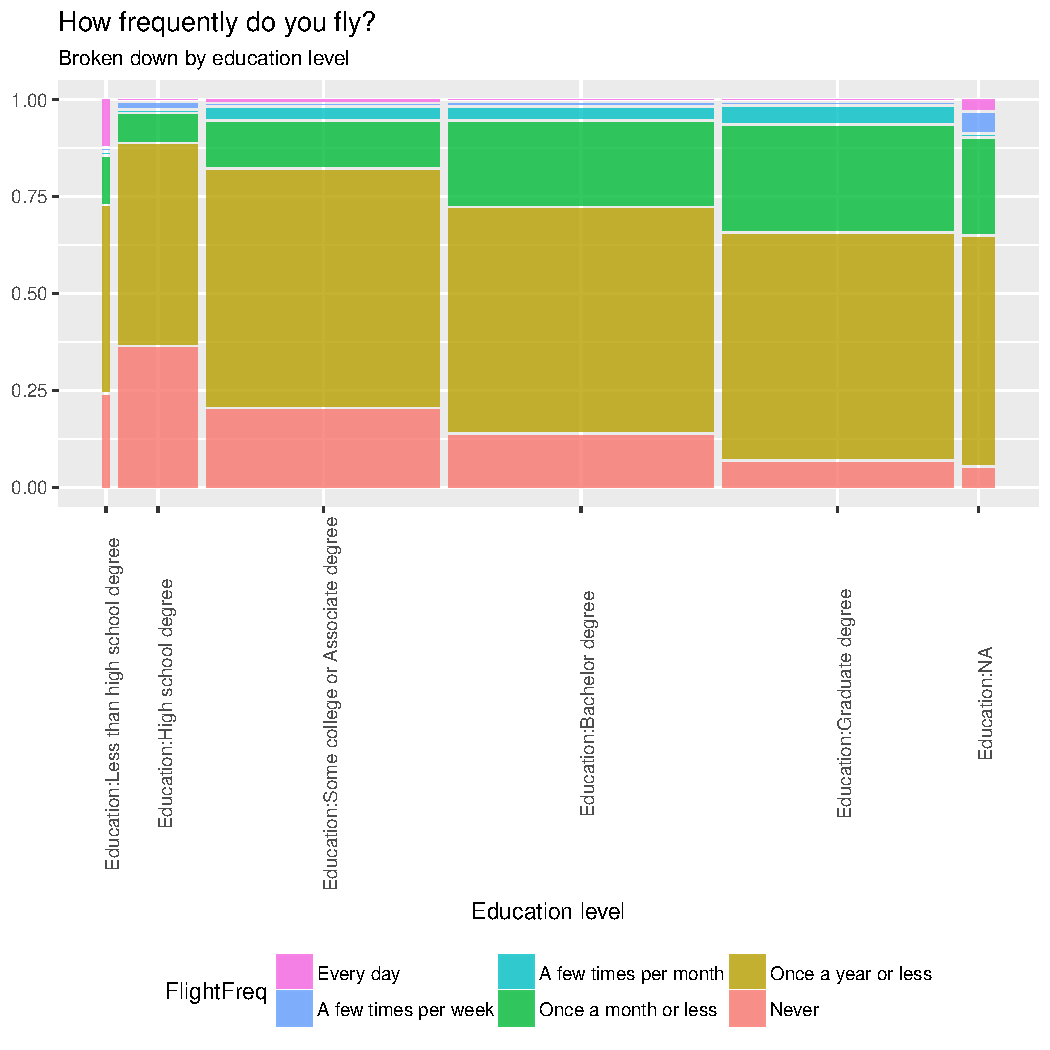
\includegraphics{flying-who2}
\label{fig: who2}
\end{figure}

\par Continuing the investigation into who is flying and how frequently they fly, Figure ~\ref{fig: who2} presents how frequently the respondents flew by education level. From the mosaic plot, we can see that the majority of respondents had some type of college education and there is a trend people flying more frequently as education level increases.

\begin{figure}[h!]
\caption{Who is flying?}
\centering
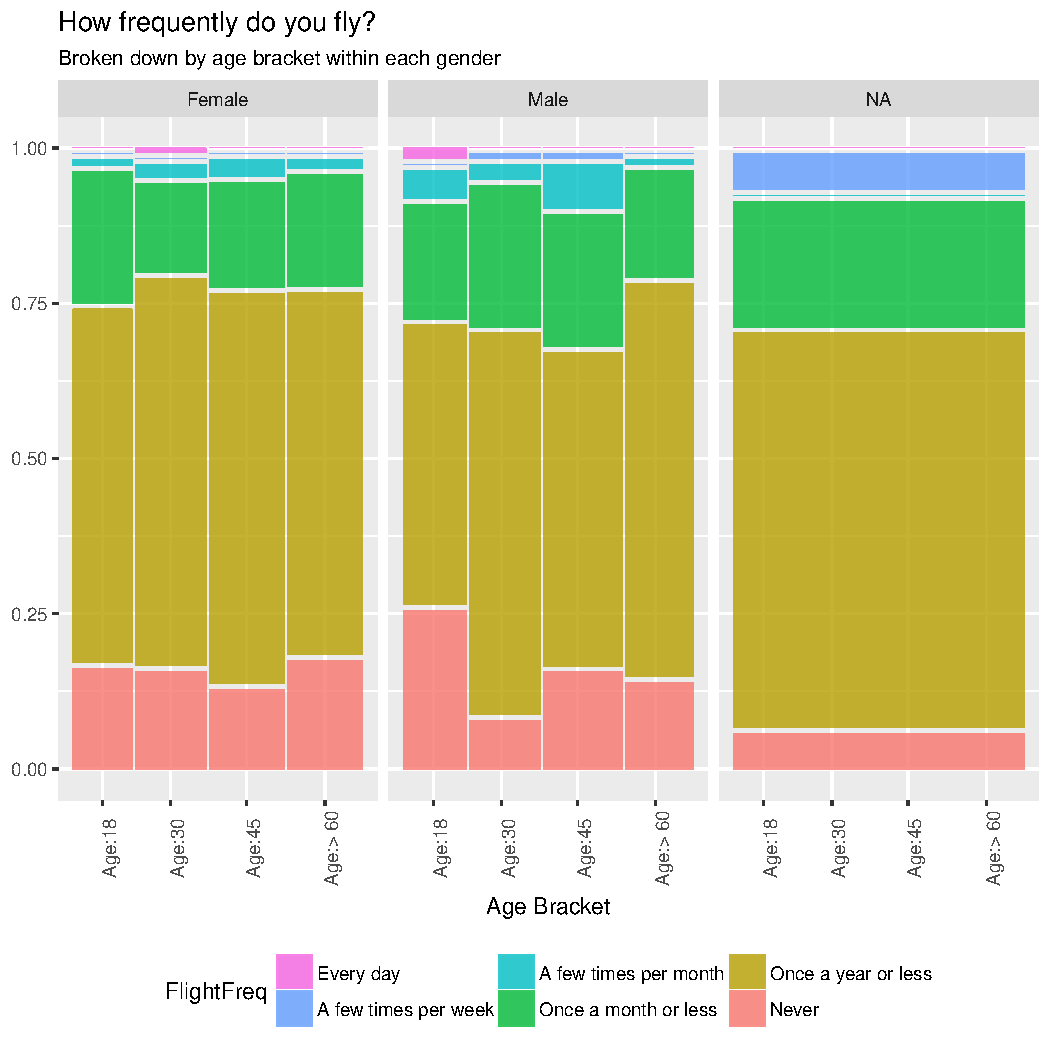
\includegraphics{flying-who3}
\label{fig: who3}
\end{figure}

\par  To add to this,  Figure ~\ref{fig: who3} shows that gender and age don't play too large of a role in how often one flies, though interestingly the largest group of those that never fly was made up of males in the age bracket 18-29.  Figure ~\ref{fig: who3} exemplifies how having mosaic plots implemented as a geom allows for the ggplot2 customization features to easily be accessed. Here, rather than partitioning into spines for the gender categories, I have faceted on gender. Statistically, this relates to conditioning on the variable on gender. The distribution that is being displayed by  Figure ~\ref{fig: who3} is f(FlightFreq, Age |Gender)




\begin{figure}[h!]
\caption{Opinions on reclining}
\centering
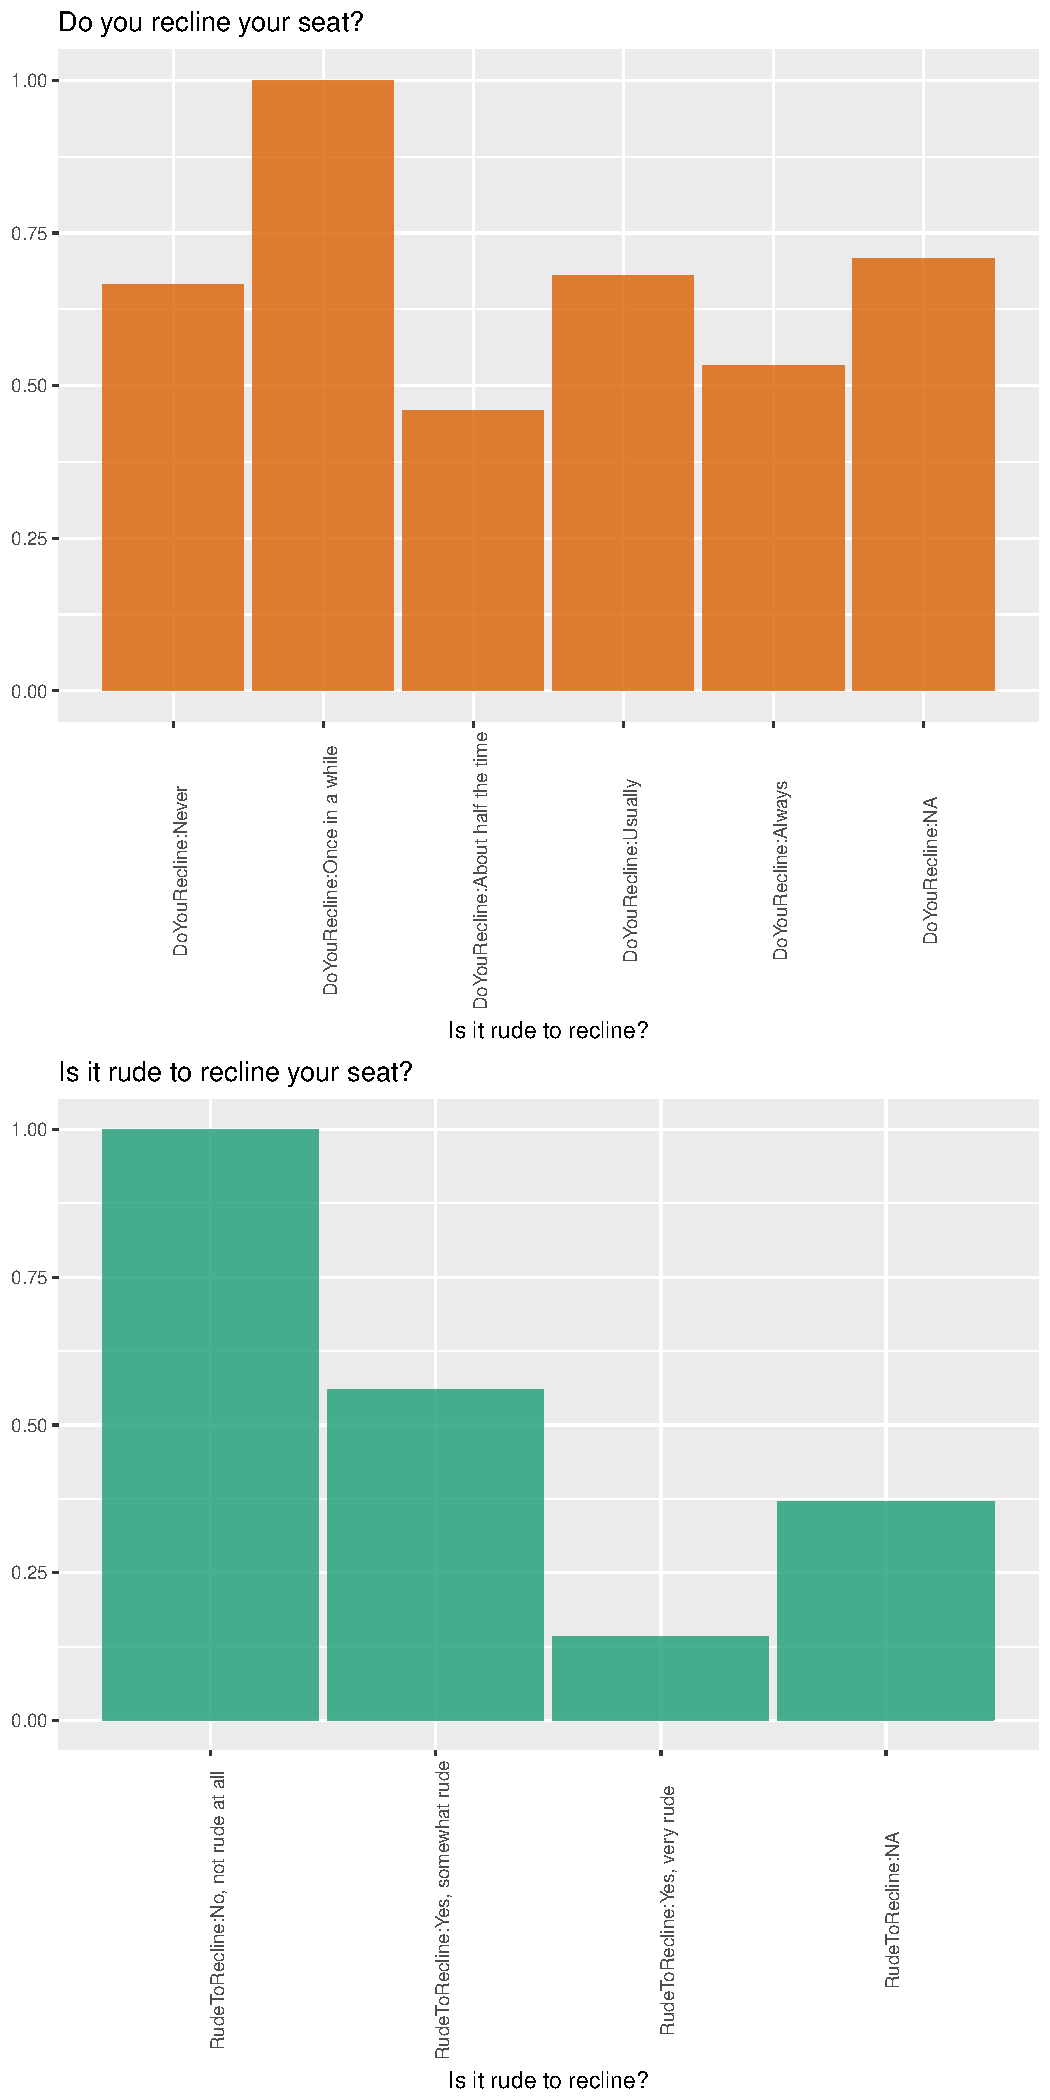
\includegraphics{flying-recline1}
\label{fig: recline1}
\end{figure}

\par Next I dove into the perceived level of rudeness of some of the more common behaviors. First up, how do the participants view "The seat recliner" and are the participants seat recliners themselves? As airlines look to shrink costs, the  airline seats appear to be shrinking as well. In the past thirty years, the average cheap seat has shrank from 18 inches wide to about 16 and a half inches wide. \citet{washpost} Has this smaller space brought strong opinions on a flight passenger's right to recline their seat? We can look at how often the participants reclined their seat and also at how rude participants believe the behavior to be. However, perhaps a more interesting question is "How often does one recline given they feel the behavior is very rude?" Figure ~\ref{fig: recline} is a breakdown of participant responses to the two questions "Do you recline?" and "Is it rude to recline?" that can allow for such types of questions to be answered. While some of the results were as expected - the more rude someone considers the act reclining, the less likely they were to recline their own chair- there were three respondents who felt it was very rude to recline your seat on an airplane, yet always reclined their own seat. The plot also lets us know that the majority of the respondents do not find it at all rude to recline your seat and are fairly evenly divided on how often they themselves recline their own seat.


\begin{figure}[h!]
\caption{Opinions on reclining}
\centering
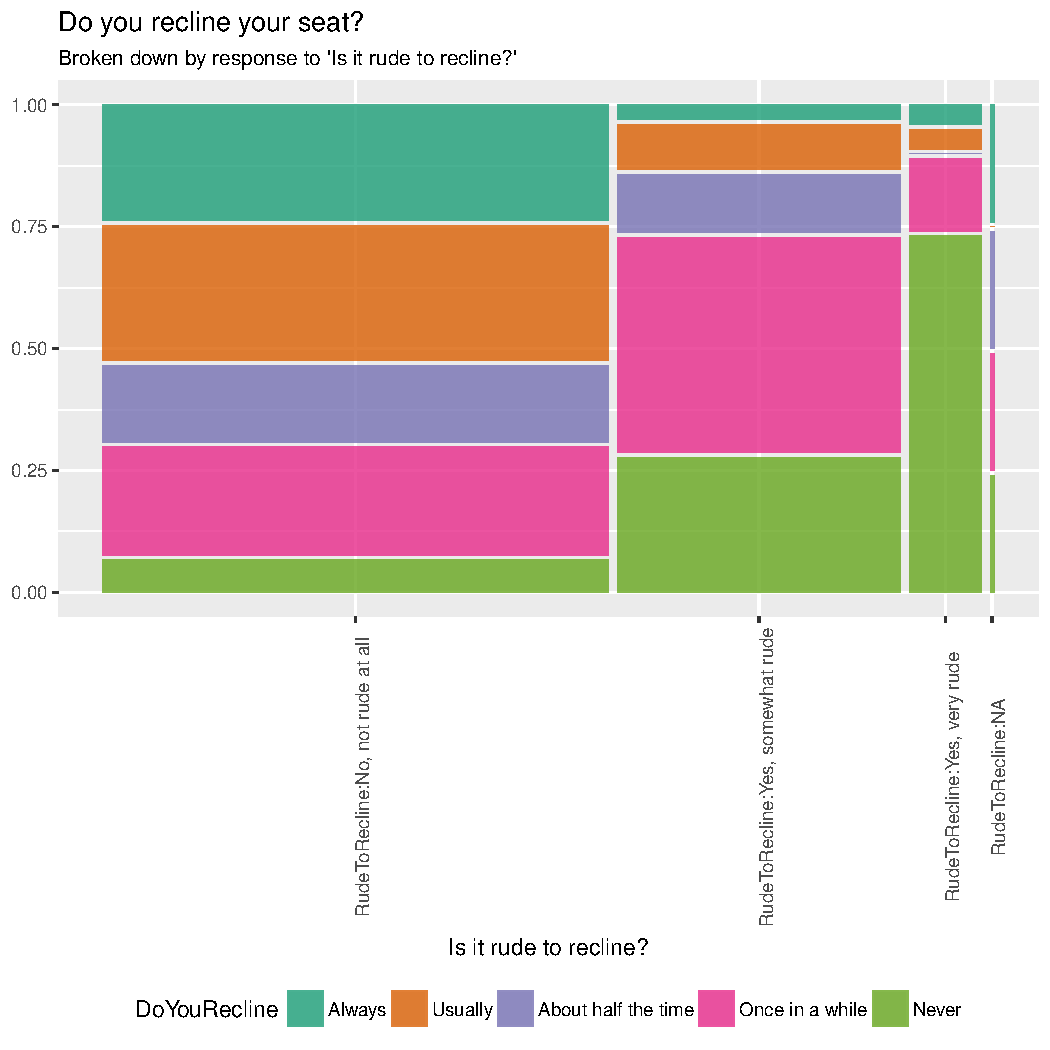
\includegraphics{flying-recline}
\label{fig: recline}
\end{figure}


\begin{figure}[h!]
\caption{Opinions on eliminating reclining}
\centering
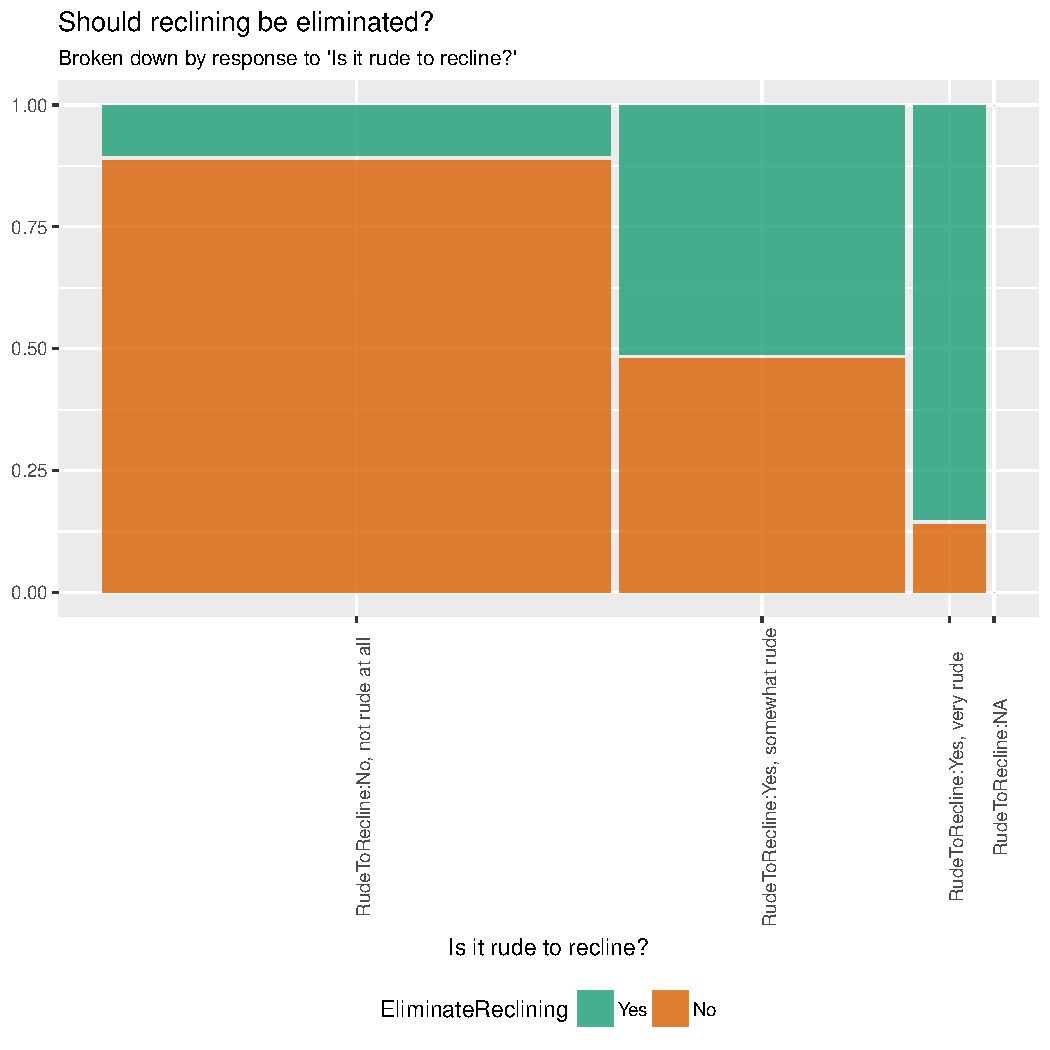
\includegraphics{flying-eliminate}
\label{fig: eliminate}
\end{figure}

\par Not a particularly surprising revelation, but Figure ~\ref{fig: eliminate} displays how the small propotion of participants that view the act of reclining your seat on an airplane as rude would also like to eliminate the option of reclining. In contrast the larger proportion that do not view the act as rude do not see a reason to eliminate the option.


\par Next, how did the participants view babies and unruly children on flights? Are there certain demographics that are more likely to be offended by their presence? Are parents less likely or more likely to be offended by other children? The firstplot adressing this topic is Figure ~\ref{fig: baby}. Here we can get an idea of how the particpiants viewed the act of bringing a baby on an aircraft. Fortunately, we see that most were not bothered, but there is a slight proportion that finds it to be very rude.

\par To see where those respondents might be coming from, the next plot looks at how the participants judged the level of rudeness of bringing a baby on board broken down by whether the participant had a child under the age of 18 and then by gender. \ref{fig: baby2} is an example of one of the other types of plots \texttt{ggmosaic} is capable of creating, a double decker plot. A modification of a mosaic plot, a double decker plot, is composed of n-1 hspines and ends with a vspine rather than alternating hspines and vspines. In ~\ref{fig: baby2}, the plot is first split horizontally by response to "Do you have a child under the age of 18?". From there each hspine is split into gender resulting in a plot where each combination of gender and child under the age of 18 is represented by a vertical bar where the width represents the proportion of that category. Lastly, each vertical bar is split vertically by the responses to "Is it rude to bring a baby on a plane?" The finished product is a plot that allows for the three variables to be presented concisely and displays how the proportions differ.


\begin{figure}[h!]
\caption{Opinions on babies on flights}
\centering
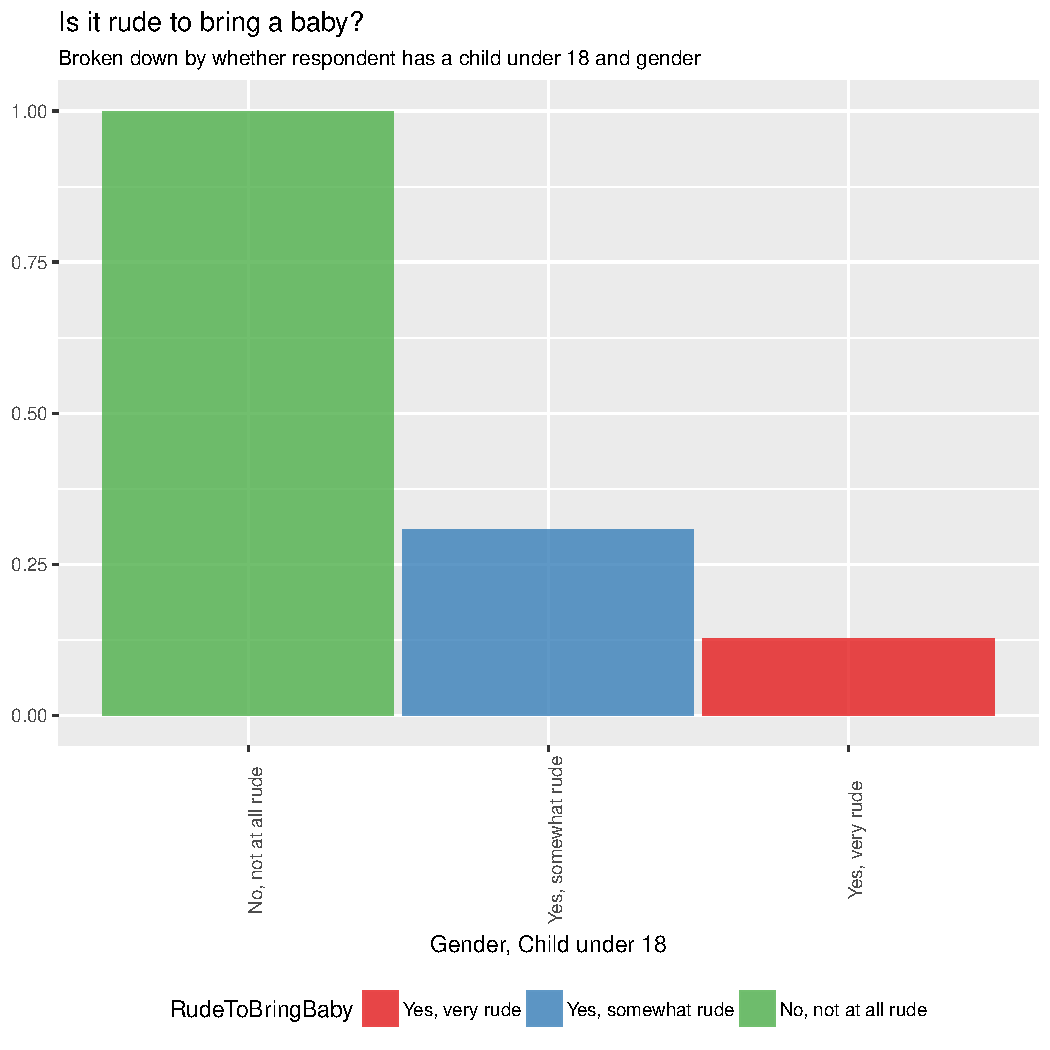
\includegraphics{flying-baby}
\label{fig: baby}
\end{figure}

\par In ~\ref{fig: baby}, we see that those without a child under the age of 18 make up the largest proportion of the respondents and they are more likely to consider bringing a baby on board as rude. Additionally, men or more likely than women to consider it rude to bring a baby on a flight.


\begin{figure}[h!]
\caption{Opinions on babies on flights}
\centering
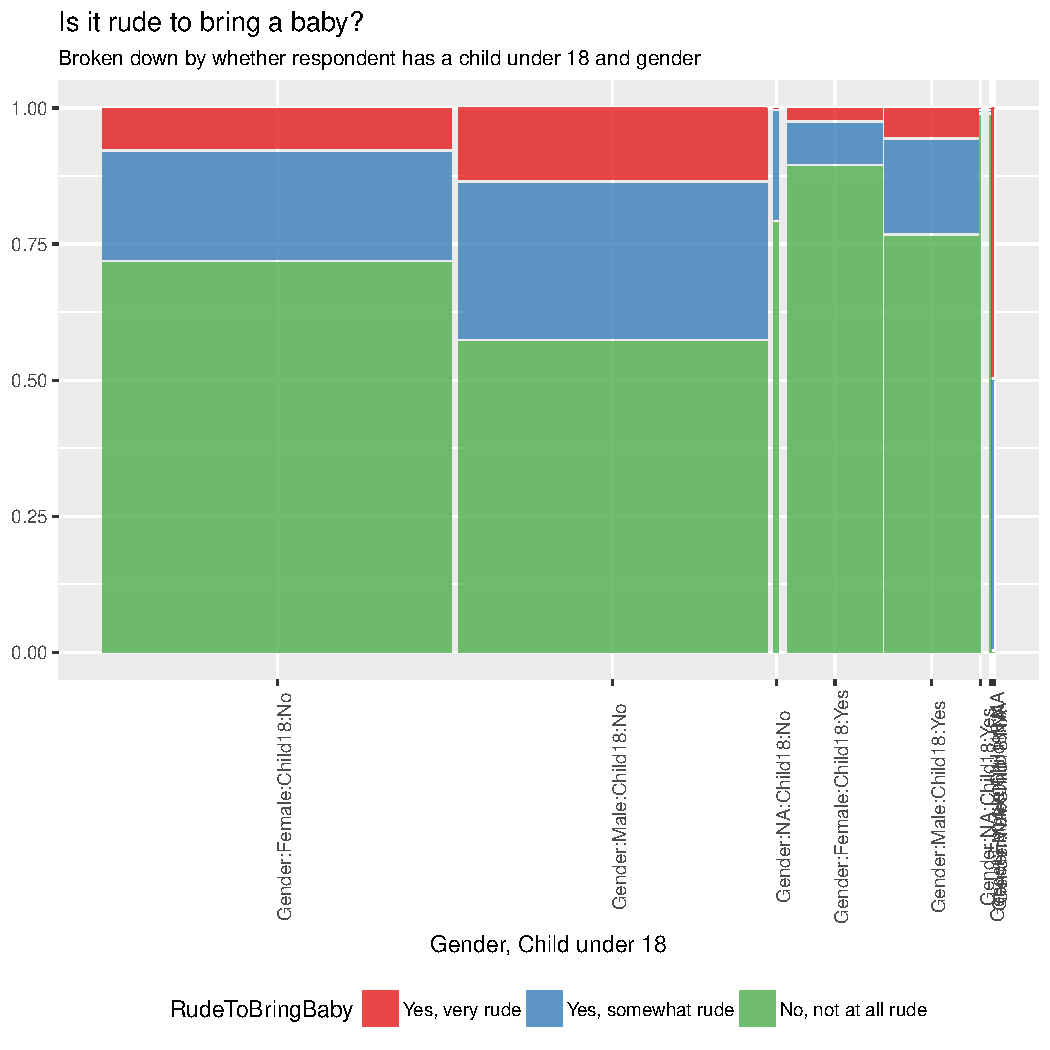
\includegraphics{flying-baby2}
\label{fig: baby2}
\end{figure}


\par The next figure, Figure ~\ref{fig: child}, looks into how the participants viewed sharing the plane ride with an unruly child. In Figure ~\ref{fig: child} we can see that the participants were likely to be bothered by an unruly child. Perhaps this has to do with the wording of the question in the SurveyMonkey, but I continued on with the analyis anyway.



\begin{figure}[h!]
\caption{Opinions on unruly children on flights}
\centering
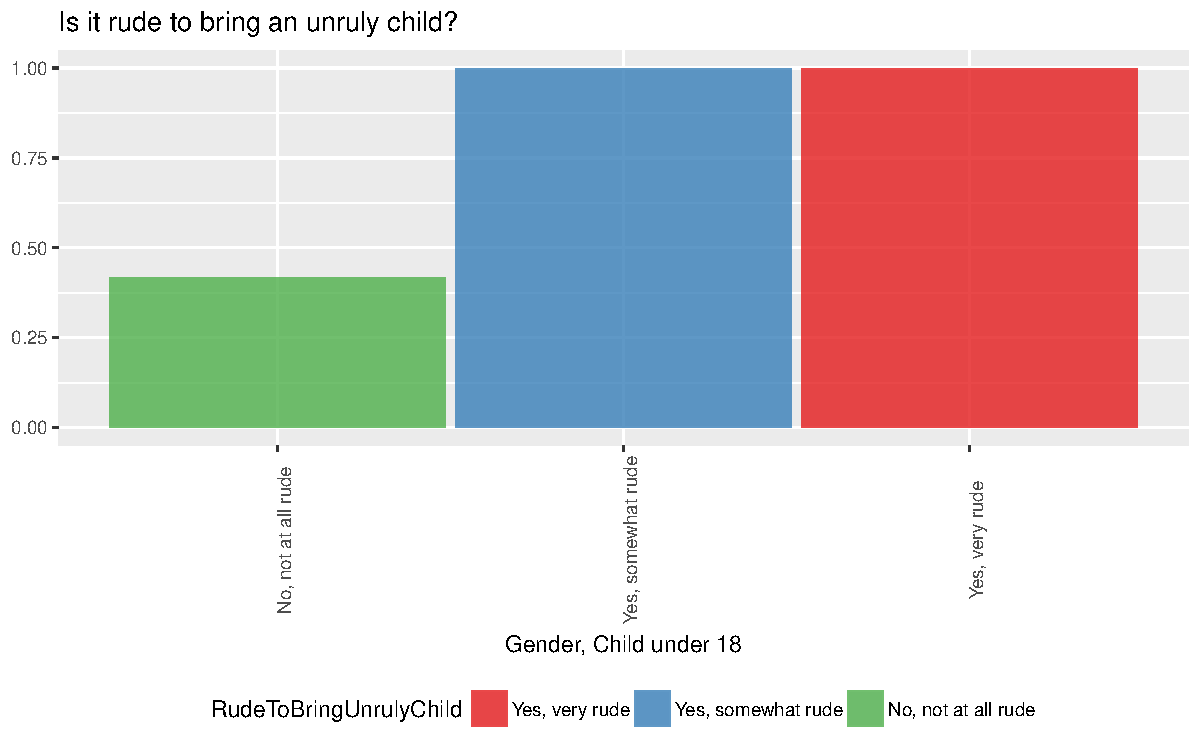
\includegraphics{flying-child}
\label{fig: child}
\end{figure}

\par To see where those opinions stemmed from, or to see if those opinions varied by gender and whether or not the participant has a child under the age of 18, Figure ~\ref{fig: child2} was created. In the double decker plot, it is clear that females are more forgiving of unruly children than males and that parents of children under the age of 18 are also more forgiving. It does, however, seem fairly clear that most find the presence of an unruly child as rude.

\begin{figure}[h!]
\caption{Opinions on unruly children on flights}
\centering
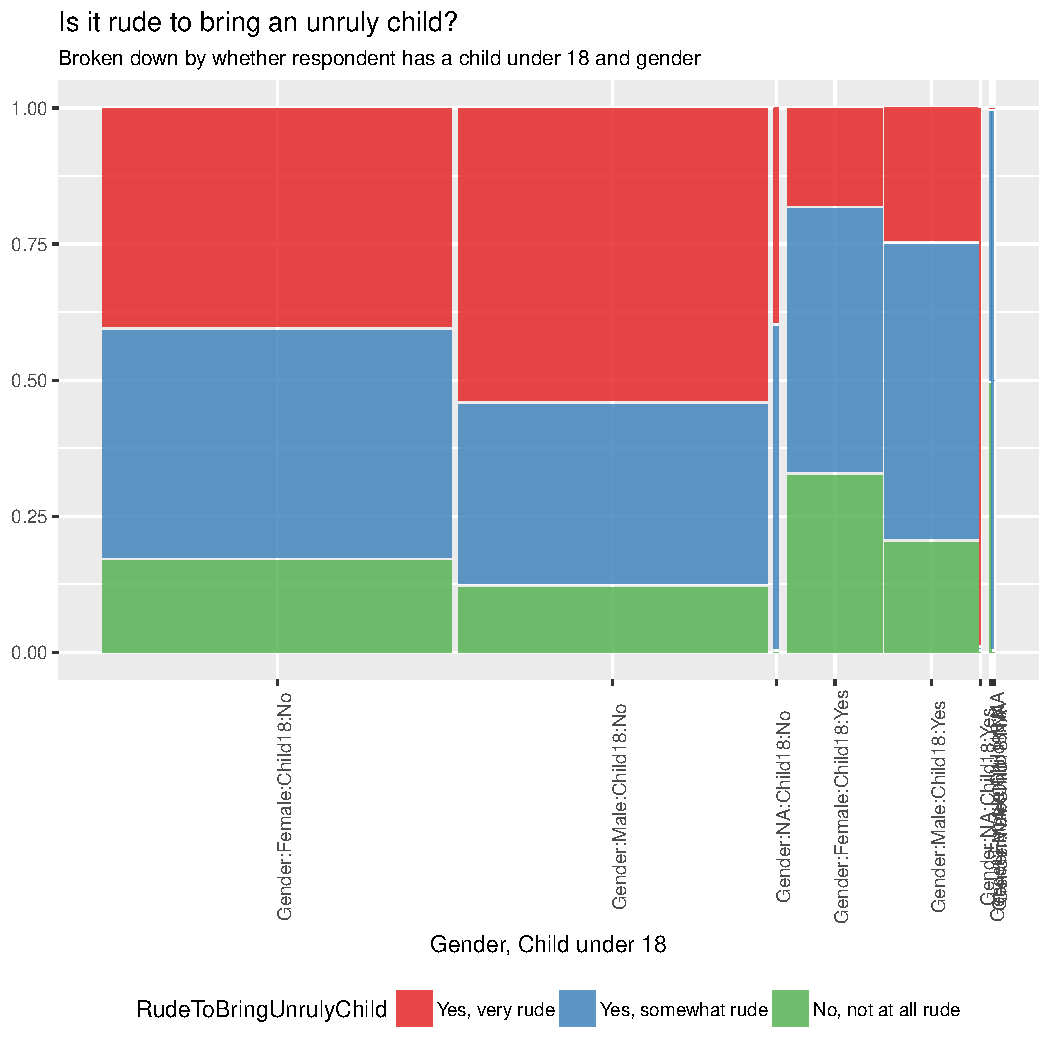
\includegraphics{flying-child2}
\label{fig: child2}
\end{figure}

\begin{figure}[h!]
\caption{Opinions on babies on flights}
\centering
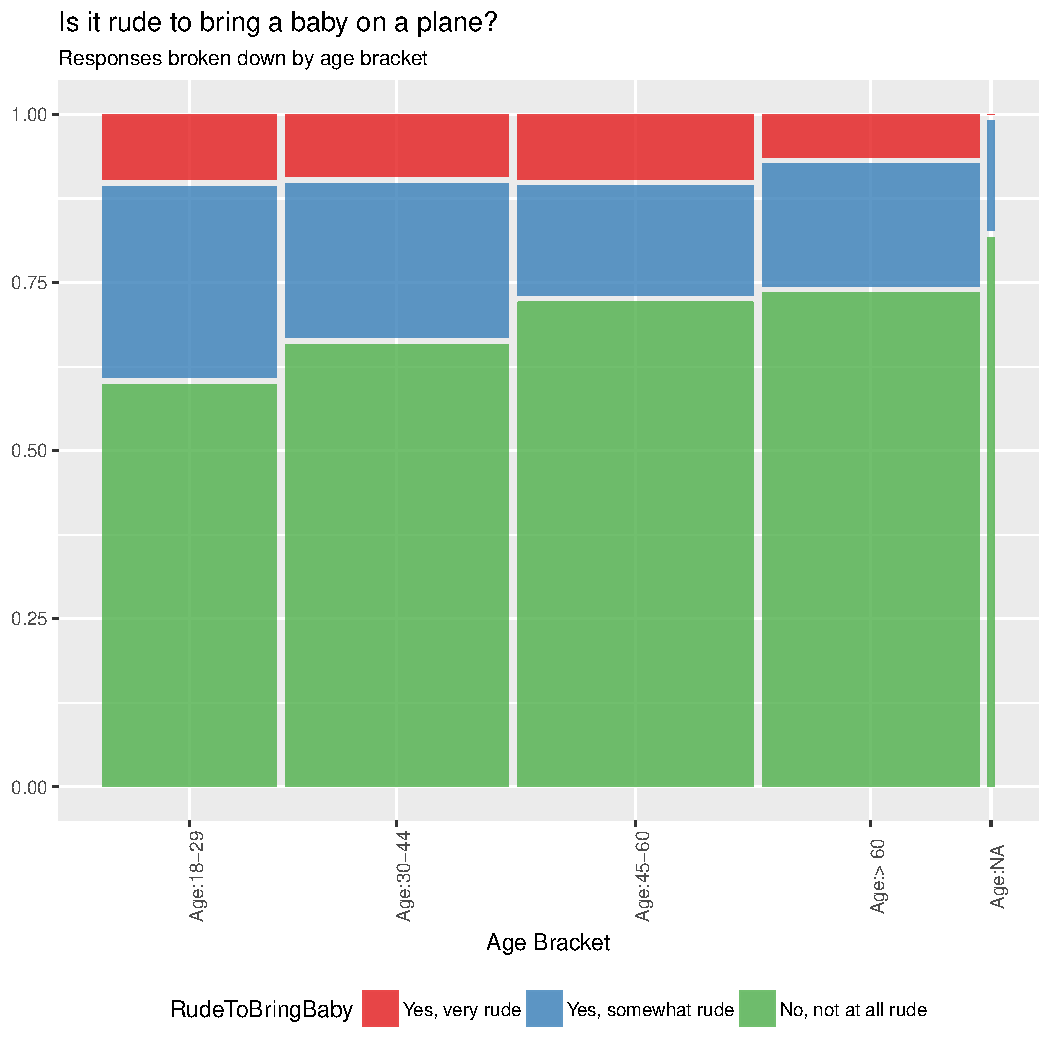
\includegraphics{flying-age_baby}
\label{fig: age_baby}
\end{figure}

\begin{figure}[h!]
\caption{Opinions on unruly children on flights}
\centering
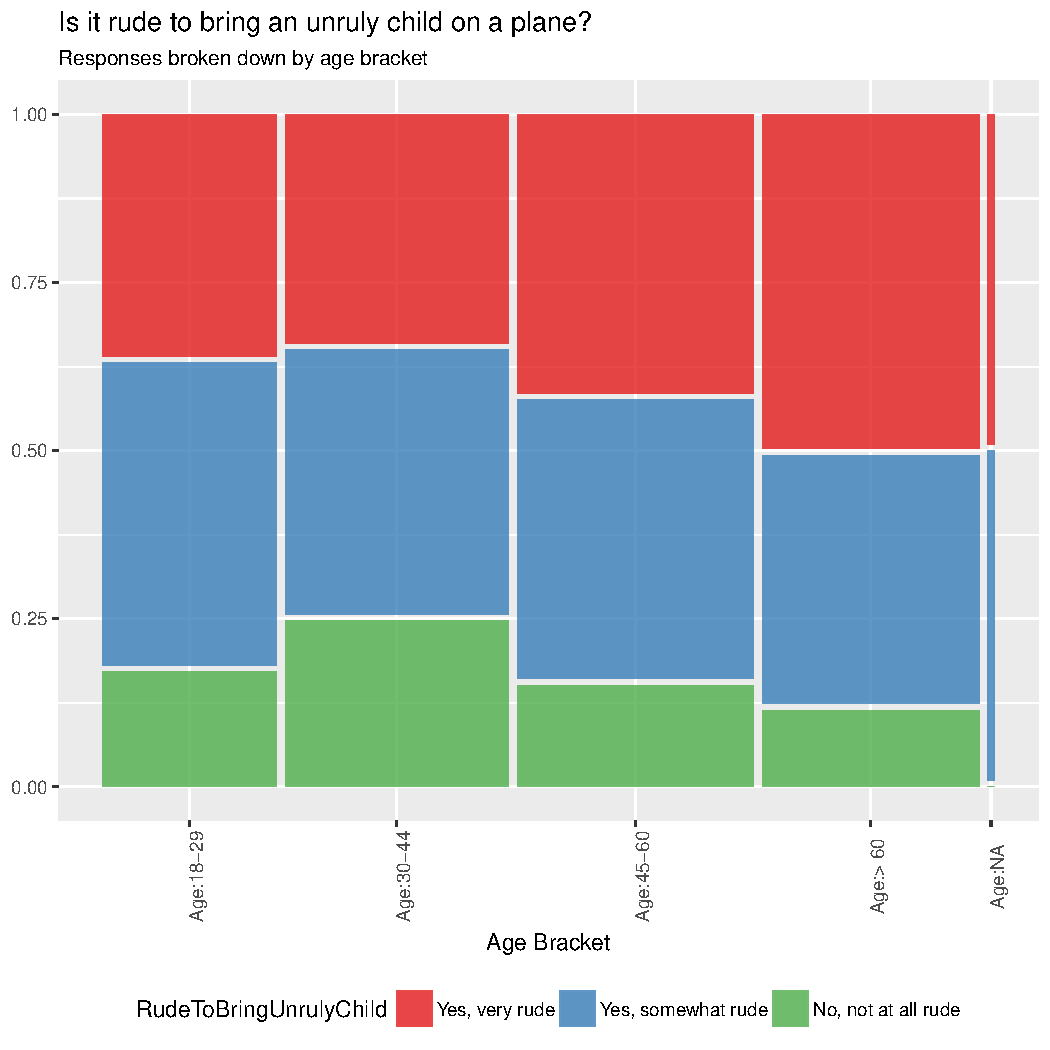
\includegraphics{flying-age_child}
\label{fig: age_child}
\end{figure}

\par To continue the investigation of how often faircraft passengers find an unruly child or baby on board as rude and how this opinion varies person to person, Figures ~\ref{fig: age_baby} and ~\ref{fig: age_child} were created. An interesting revelation brought about by these two plots is that while those older seem to be less likely to be bothered by a baby being on a flight, they are more likely to be upset by an unruly child.

\section*{Conclusion}


\par After exploring the data a bit more, it is clear that there does not seem to be a general consensus on what passengers perceive to be acceptable behavior on an airplane. The use of mosaic plots aided in the exploration of how certain opinions or behaviors are related.
%----------------------------------------------------------------------------------------
%	REFERENCE LIST
%----------------------------------------------------------------------------------------
\bibliographystyle{asa.bst}
%\biboptions{authoryear}
\bibliography{references}

%----------------------------------------------------------------------------------------


\end{document}
